\documentclass{article}
\usepackage{iclr2027_conference,times}
\renewcommand{\ttdefault}{cmtt}
%%%%% NEW MATH DEFINITIONS %%%%%

\usepackage{amsmath,amsfonts,bm}

% Mark sections of captions for referring to divisions of figures
\newcommand{\figleft}{{\em (Left)}}
\newcommand{\figcenter}{{\em (Center)}}
\newcommand{\figright}{{\em (Right)}}
\newcommand{\figtop}{{\em (Top)}}
\newcommand{\figbottom}{{\em (Bottom)}}
\newcommand{\captiona}{{\em (a)}}
\newcommand{\captionb}{{\em (b)}}
\newcommand{\captionc}{{\em (c)}}
\newcommand{\captiond}{{\em (d)}}

% Highlight a newly defined term
\newcommand{\newterm}[1]{{\bf #1}}


% Figure reference, lower-case.
\def\figref#1{figure~\ref{#1}}
% Figure reference, capital. For start of sentence
\def\Figref#1{Figure~\ref{#1}}
\def\twofigref#1#2{figures \ref{#1} and \ref{#2}}
\def\quadfigref#1#2#3#4{figures \ref{#1}, \ref{#2}, \ref{#3} and \ref{#4}}
% Section reference, lower-case.
\def\secref#1{section~\ref{#1}}
% Section reference, capital.
\def\Secref#1{Section~\ref{#1}}
% Reference to two sections.
\def\twosecrefs#1#2{sections \ref{#1} and \ref{#2}}
% Reference to three sections.
\def\secrefs#1#2#3{sections \ref{#1}, \ref{#2} and \ref{#3}}
% Reference to an equation, lower-case.
\def\eqref#1{equation~\ref{#1}}
% Reference to an equation, upper case
\def\Eqref#1{Equation~\ref{#1}}
% A raw reference to an equation---avoid using if possible
\def\plaineqref#1{\ref{#1}}
% Reference to a chapter, lower-case.
\def\chapref#1{chapter~\ref{#1}}
% Reference to an equation, upper case.
\def\Chapref#1{Chapter~\ref{#1}}
% Reference to a range of chapters
\def\rangechapref#1#2{chapters\ref{#1}--\ref{#2}}
% Reference to an algorithm, lower-case.
\def\algref#1{algorithm~\ref{#1}}
% Reference to an algorithm, upper case.
\def\Algref#1{Algorithm~\ref{#1}}
\def\twoalgref#1#2{algorithms \ref{#1} and \ref{#2}}
\def\Twoalgref#1#2{Algorithms \ref{#1} and \ref{#2}}
% Reference to a part, lower case
\def\partref#1{part~\ref{#1}}
% Reference to a part, upper case
\def\Partref#1{Part~\ref{#1}}
\def\twopartref#1#2{parts \ref{#1} and \ref{#2}}

\def\ceil#1{\lceil #1 \rceil}
\def\floor#1{\lfloor #1 \rfloor}
\def\1{\bm{1}}
\newcommand{\train}{\mathcal{D}}
\newcommand{\valid}{\mathcal{D_{\mathrm{valid}}}}
\newcommand{\test}{\mathcal{D_{\mathrm{test}}}}

\def\eps{{\epsilon}}


% Random variables
\def\reta{{\textnormal{$\eta$}}}
\def\ra{{\textnormal{a}}}
\def\rb{{\textnormal{b}}}
\def\rc{{\textnormal{c}}}
\def\rd{{\textnormal{d}}}
\def\re{{\textnormal{e}}}
\def\rf{{\textnormal{f}}}
\def\rg{{\textnormal{g}}}
\def\rh{{\textnormal{h}}}
\def\ri{{\textnormal{i}}}
\def\rj{{\textnormal{j}}}
\def\rk{{\textnormal{k}}}
\def\rl{{\textnormal{l}}}
% rm is already a command, just don't name any random variables m
\def\rn{{\textnormal{n}}}
\def\ro{{\textnormal{o}}}
\def\rp{{\textnormal{p}}}
\def\rq{{\textnormal{q}}}
\def\rr{{\textnormal{r}}}
\def\rs{{\textnormal{s}}}
\def\rt{{\textnormal{t}}}
\def\ru{{\textnormal{u}}}
\def\rv{{\textnormal{v}}}
\def\rw{{\textnormal{w}}}
\def\rx{{\textnormal{x}}}
\def\ry{{\textnormal{y}}}
\def\rz{{\textnormal{z}}}

% Random vectors
\def\rvepsilon{{\mathbf{\epsilon}}}
\def\rvtheta{{\mathbf{\theta}}}
\def\rva{{\mathbf{a}}}
\def\rvb{{\mathbf{b}}}
\def\rvc{{\mathbf{c}}}
\def\rvd{{\mathbf{d}}}
\def\rve{{\mathbf{e}}}
\def\rvf{{\mathbf{f}}}
\def\rvg{{\mathbf{g}}}
\def\rvh{{\mathbf{h}}}
\def\rvu{{\mathbf{i}}}
\def\rvj{{\mathbf{j}}}
\def\rvk{{\mathbf{k}}}
\def\rvl{{\mathbf{l}}}
\def\rvm{{\mathbf{m}}}
\def\rvn{{\mathbf{n}}}
\def\rvo{{\mathbf{o}}}
\def\rvp{{\mathbf{p}}}
\def\rvq{{\mathbf{q}}}
\def\rvr{{\mathbf{r}}}
\def\rvs{{\mathbf{s}}}
\def\rvt{{\mathbf{t}}}
\def\rvu{{\mathbf{u}}}
\def\rvv{{\mathbf{v}}}
\def\rvw{{\mathbf{w}}}
\def\rvx{{\mathbf{x}}}
\def\rvy{{\mathbf{y}}}
\def\rvz{{\mathbf{z}}}

% Elements of random vectors
\def\erva{{\textnormal{a}}}
\def\ervb{{\textnormal{b}}}
\def\ervc{{\textnormal{c}}}
\def\ervd{{\textnormal{d}}}
\def\erve{{\textnormal{e}}}
\def\ervf{{\textnormal{f}}}
\def\ervg{{\textnormal{g}}}
\def\ervh{{\textnormal{h}}}
\def\ervi{{\textnormal{i}}}
\def\ervj{{\textnormal{j}}}
\def\ervk{{\textnormal{k}}}
\def\ervl{{\textnormal{l}}}
\def\ervm{{\textnormal{m}}}
\def\ervn{{\textnormal{n}}}
\def\ervo{{\textnormal{o}}}
\def\ervp{{\textnormal{p}}}
\def\ervq{{\textnormal{q}}}
\def\ervr{{\textnormal{r}}}
\def\ervs{{\textnormal{s}}}
\def\ervt{{\textnormal{t}}}
\def\ervu{{\textnormal{u}}}
\def\ervv{{\textnormal{v}}}
\def\ervw{{\textnormal{w}}}
\def\ervx{{\textnormal{x}}}
\def\ervy{{\textnormal{y}}}
\def\ervz{{\textnormal{z}}}

% Random matrices
\def\rmA{{\mathbf{A}}}
\def\rmB{{\mathbf{B}}}
\def\rmC{{\mathbf{C}}}
\def\rmD{{\mathbf{D}}}
\def\rmE{{\mathbf{E}}}
\def\rmF{{\mathbf{F}}}
\def\rmG{{\mathbf{G}}}
\def\rmH{{\mathbf{H}}}
\def\rmI{{\mathbf{I}}}
\def\rmJ{{\mathbf{J}}}
\def\rmK{{\mathbf{K}}}
\def\rmL{{\mathbf{L}}}
\def\rmM{{\mathbf{M}}}
\def\rmN{{\mathbf{N}}}
\def\rmO{{\mathbf{O}}}
\def\rmP{{\mathbf{P}}}
\def\rmQ{{\mathbf{Q}}}
\def\rmR{{\mathbf{R}}}
\def\rmS{{\mathbf{S}}}
\def\rmT{{\mathbf{T}}}
\def\rmU{{\mathbf{U}}}
\def\rmV{{\mathbf{V}}}
\def\rmW{{\mathbf{W}}}
\def\rmX{{\mathbf{X}}}
\def\rmY{{\mathbf{Y}}}
\def\rmZ{{\mathbf{Z}}}

% Elements of random matrices
\def\ermA{{\textnormal{A}}}
\def\ermB{{\textnormal{B}}}
\def\ermC{{\textnormal{C}}}
\def\ermD{{\textnormal{D}}}
\def\ermE{{\textnormal{E}}}
\def\ermF{{\textnormal{F}}}
\def\ermG{{\textnormal{G}}}
\def\ermH{{\textnormal{H}}}
\def\ermI{{\textnormal{I}}}
\def\ermJ{{\textnormal{J}}}
\def\ermK{{\textnormal{K}}}
\def\ermL{{\textnormal{L}}}
\def\ermM{{\textnormal{M}}}
\def\ermN{{\textnormal{N}}}
\def\ermO{{\textnormal{O}}}
\def\ermP{{\textnormal{P}}}
\def\ermQ{{\textnormal{Q}}}
\def\ermR{{\textnormal{R}}}
\def\ermS{{\textnormal{S}}}
\def\ermT{{\textnormal{T}}}
\def\ermU{{\textnormal{U}}}
\def\ermV{{\textnormal{V}}}
\def\ermW{{\textnormal{W}}}
\def\ermX{{\textnormal{X}}}
\def\ermY{{\textnormal{Y}}}
\def\ermZ{{\textnormal{Z}}}

% Vectors
\def\vzero{{\bm{0}}}
\def\vone{{\bm{1}}}
\def\vmu{{\bm{\mu}}}
\def\vtheta{{\bm{\theta}}}
\def\va{{\bm{a}}}
\def\vb{{\bm{b}}}
\def\vc{{\bm{c}}}
\def\vd{{\bm{d}}}
\def\ve{{\bm{e}}}
\def\vf{{\bm{f}}}
\def\vg{{\bm{g}}}
\def\vh{{\bm{h}}}
\def\vi{{\bm{i}}}
\def\vj{{\bm{j}}}
\def\vk{{\bm{k}}}
\def\vl{{\bm{l}}}
\def\vm{{\bm{m}}}
\def\vn{{\bm{n}}}
\def\vo{{\bm{o}}}
\def\vp{{\bm{p}}}
\def\vq{{\bm{q}}}
\def\vr{{\bm{r}}}
\def\vs{{\bm{s}}}
\def\vt{{\bm{t}}}
\def\vu{{\bm{u}}}
\def\vv{{\bm{v}}}
\def\vw{{\bm{w}}}
\def\vx{{\bm{x}}}
\def\vy{{\bm{y}}}
\def\vz{{\bm{z}}}

% Elements of vectors
\def\evalpha{{\alpha}}
\def\evbeta{{\beta}}
\def\evepsilon{{\epsilon}}
\def\evlambda{{\lambda}}
\def\evomega{{\omega}}
\def\evmu{{\mu}}
\def\evpsi{{\psi}}
\def\evsigma{{\sigma}}
\def\evtheta{{\theta}}
\def\eva{{a}}
\def\evb{{b}}
\def\evc{{c}}
\def\evd{{d}}
\def\eve{{e}}
\def\evf{{f}}
\def\evg{{g}}
\def\evh{{h}}
\def\evi{{i}}
\def\evj{{j}}
\def\evk{{k}}
\def\evl{{l}}
\def\evm{{m}}
\def\evn{{n}}
\def\evo{{o}}
\def\evp{{p}}
\def\evq{{q}}
\def\evr{{r}}
\def\evs{{s}}
\def\evt{{t}}
\def\evu{{u}}
\def\evv{{v}}
\def\evw{{w}}
\def\evx{{x}}
\def\evy{{y}}
\def\evz{{z}}

% Matrix
\def\mA{{\bm{A}}}
\def\mB{{\bm{B}}}
\def\mC{{\bm{C}}}
\def\mD{{\bm{D}}}
\def\mE{{\bm{E}}}
\def\mF{{\bm{F}}}
\def\mG{{\bm{G}}}
\def\mH{{\bm{H}}}
\def\mI{{\bm{I}}}
\def\mJ{{\bm{J}}}
\def\mK{{\bm{K}}}
\def\mL{{\bm{L}}}
\def\mM{{\bm{M}}}
\def\mN{{\bm{N}}}
\def\mO{{\bm{O}}}
\def\mP{{\bm{P}}}
\def\mQ{{\bm{Q}}}
\def\mR{{\bm{R}}}
\def\mS{{\bm{S}}}
\def\mT{{\bm{T}}}
\def\mU{{\bm{U}}}
\def\mV{{\bm{V}}}
\def\mW{{\bm{W}}}
\def\mX{{\bm{X}}}
\def\mY{{\bm{Y}}}
\def\mZ{{\bm{Z}}}
\def\mBeta{{\bm{\beta}}}
\def\mPhi{{\bm{\Phi}}}
\def\mLambda{{\bm{\Lambda}}}
\def\mSigma{{\bm{\Sigma}}}

% Tensor
\DeclareMathAlphabet{\mathsfit}{\encodingdefault}{\sfdefault}{m}{sl}
\SetMathAlphabet{\mathsfit}{bold}{\encodingdefault}{\sfdefault}{bx}{n}
\newcommand{\tens}[1]{\bm{\mathsfit{#1}}}
\def\tA{{\tens{A}}}
\def\tB{{\tens{B}}}
\def\tC{{\tens{C}}}
\def\tD{{\tens{D}}}
\def\tE{{\tens{E}}}
\def\tF{{\tens{F}}}
\def\tG{{\tens{G}}}
\def\tH{{\tens{H}}}
\def\tI{{\tens{I}}}
\def\tJ{{\tens{J}}}
\def\tK{{\tens{K}}}
\def\tL{{\tens{L}}}
\def\tM{{\tens{M}}}
\def\tN{{\tens{N}}}
\def\tO{{\tens{O}}}
\def\tP{{\tens{P}}}
\def\tQ{{\tens{Q}}}
\def\tR{{\tens{R}}}
\def\tS{{\tens{S}}}
\def\tT{{\tens{T}}}
\def\tU{{\tens{U}}}
\def\tV{{\tens{V}}}
\def\tW{{\tens{W}}}
\def\tX{{\tens{X}}}
\def\tY{{\tens{Y}}}
\def\tZ{{\tens{Z}}}


% Graph
\def\gA{{\mathcal{A}}}
\def\gB{{\mathcal{B}}}
\def\gC{{\mathcal{C}}}
\def\gD{{\mathcal{D}}}
\def\gE{{\mathcal{E}}}
\def\gF{{\mathcal{F}}}
\def\gG{{\mathcal{G}}}
\def\gH{{\mathcal{H}}}
\def\gI{{\mathcal{I}}}
\def\gJ{{\mathcal{J}}}
\def\gK{{\mathcal{K}}}
\def\gL{{\mathcal{L}}}
\def\gM{{\mathcal{M}}}
\def\gN{{\mathcal{N}}}
\def\gO{{\mathcal{O}}}
\def\gP{{\mathcal{P}}}
\def\gQ{{\mathcal{Q}}}
\def\gR{{\mathcal{R}}}
\def\gS{{\mathcal{S}}}
\def\gT{{\mathcal{T}}}
\def\gU{{\mathcal{U}}}
\def\gV{{\mathcal{V}}}
\def\gW{{\mathcal{W}}}
\def\gX{{\mathcal{X}}}
\def\gY{{\mathcal{Y}}}
\def\gZ{{\mathcal{Z}}}

% Sets
\def\sA{{\mathbb{A}}}
\def\sB{{\mathbb{B}}}
\def\sC{{\mathbb{C}}}
\def\sD{{\mathbb{D}}}
% Don't use a set called E, because this would be the same as our symbol
% for expectation.
\def\sF{{\mathbb{F}}}
\def\sG{{\mathbb{G}}}
\def\sH{{\mathbb{H}}}
\def\sI{{\mathbb{I}}}
\def\sJ{{\mathbb{J}}}
\def\sK{{\mathbb{K}}}
\def\sL{{\mathbb{L}}}
\def\sM{{\mathbb{M}}}
\def\sN{{\mathbb{N}}}
\def\sO{{\mathbb{O}}}
\def\sP{{\mathbb{P}}}
\def\sQ{{\mathbb{Q}}}
\def\sR{{\mathbb{R}}}
\def\sS{{\mathbb{S}}}
\def\sT{{\mathbb{T}}}
\def\sU{{\mathbb{U}}}
\def\sV{{\mathbb{V}}}
\def\sW{{\mathbb{W}}}
\def\sX{{\mathbb{X}}}
\def\sY{{\mathbb{Y}}}
\def\sZ{{\mathbb{Z}}}

% Entries of a matrix
\def\emLambda{{\Lambda}}
\def\emA{{A}}
\def\emB{{B}}
\def\emC{{C}}
\def\emD{{D}}
\def\emE{{E}}
\def\emF{{F}}
\def\emG{{G}}
\def\emH{{H}}
\def\emI{{I}}
\def\emJ{{J}}
\def\emK{{K}}
\def\emL{{L}}
\def\emM{{M}}
\def\emN{{N}}
\def\emO{{O}}
\def\emP{{P}}
\def\emQ{{Q}}
\def\emR{{R}}
\def\emS{{S}}
\def\emT{{T}}
\def\emU{{U}}
\def\emV{{V}}
\def\emW{{W}}
\def\emX{{X}}
\def\emY{{Y}}
\def\emZ{{Z}}
\def\emSigma{{\Sigma}}

% entries of a tensor
% Same font as tensor, without \bm wrapper
\newcommand{\etens}[1]{\mathsfit{#1}}
\def\etLambda{{\etens{\Lambda}}}
\def\etA{{\etens{A}}}
\def\etB{{\etens{B}}}
\def\etC{{\etens{C}}}
\def\etD{{\etens{D}}}
\def\etE{{\etens{E}}}
\def\etF{{\etens{F}}}
\def\etG{{\etens{G}}}
\def\etH{{\etens{H}}}
\def\etI{{\etens{I}}}
\def\etJ{{\etens{J}}}
\def\etK{{\etens{K}}}
\def\etL{{\etens{L}}}
\def\etM{{\etens{M}}}
\def\etN{{\etens{N}}}
\def\etO{{\etens{O}}}
\def\etP{{\etens{P}}}
\def\etQ{{\etens{Q}}}
\def\etR{{\etens{R}}}
\def\etS{{\etens{S}}}
\def\etT{{\etens{T}}}
\def\etU{{\etens{U}}}
\def\etV{{\etens{V}}}
\def\etW{{\etens{W}}}
\def\etX{{\etens{X}}}
\def\etY{{\etens{Y}}}
\def\etZ{{\etens{Z}}}

% The true underlying data generating distribution
\newcommand{\pdata}{p_{\rm{data}}}
% The empirical distribution defined by the training set
\newcommand{\ptrain}{\hat{p}_{\rm{data}}}
\newcommand{\Ptrain}{\hat{P}_{\rm{data}}}
% The model distribution
\newcommand{\pmodel}{p_{\rm{model}}}
\newcommand{\Pmodel}{P_{\rm{model}}}
\newcommand{\ptildemodel}{\tilde{p}_{\rm{model}}}
% Stochastic autoencoder distributions
\newcommand{\pencode}{p_{\rm{encoder}}}
\newcommand{\pdecode}{p_{\rm{decoder}}}
\newcommand{\precons}{p_{\rm{reconstruct}}}

\newcommand{\laplace}{\mathrm{Laplace}} % Laplace distribution

\newcommand{\E}{\mathbb{E}}
\newcommand{\Ls}{\mathcal{L}}
\newcommand{\R}{\mathbb{R}}
\newcommand{\emp}{\tilde{p}}
\newcommand{\lr}{\alpha}
\newcommand{\reg}{\lambda}
\newcommand{\rect}{\mathrm{rectifier}}
\newcommand{\softmax}{\mathrm{softmax}}
\newcommand{\sigmoid}{\sigma}
\newcommand{\softplus}{\zeta}
\newcommand{\KL}{D_{\mathrm{KL}}}
\newcommand{\Var}{\mathrm{Var}}
\newcommand{\standarderror}{\mathrm{SE}}
\newcommand{\Cov}{\mathrm{Cov}}
% Wolfram Mathworld says $L^2$ is for function spaces and $\ell^2$ is for vectors
% But then they seem to use $L^2$ for vectors throughout the site, and so does
% wikipedia.
\newcommand{\normlzero}{L^0}
\newcommand{\normlone}{L^1}
\newcommand{\normltwo}{L^2}
\newcommand{\normlp}{L^p}
\newcommand{\normmax}{L^\infty}

\newcommand{\parents}{Pa} % See usage in notation.tex. Chosen to match Daphne's book.

\DeclareMathOperator*{\argmax}{arg\,max}
\DeclareMathOperator*{\argmin}{arg\,min}

\DeclareMathOperator{\sign}{sign}
\DeclareMathOperator{\Tr}{Tr}
\let\ab\allowbreak


\usepackage{hyperref}
\usepackage{url}
\usepackage{booktabs}
\usepackage{tabularx}
\usepackage{array}
\usepackage{graphicx}
\usepackage{float}
\usepackage{subcaption}
\usepackage{amsmath,amssymb,amsfonts,amsthm}
\usepackage{bm}
\usepackage{xcolor}
\usepackage{listings}

\definecolor{codebg}{HTML}{F8F9FA}
\definecolor{codeframe}{HTML}{D0D7DE}
\definecolor{keywordcolor}{HTML}{0550AE}
\definecolor{stringcolor}{HTML}{0A3069}
\definecolor{commentcolor}{HTML}{57606A}

\lstset{
    backgroundcolor=\color{codebg},
    basicstyle=\ttfamily\scriptsize\color{black},
    keywordstyle=\color{keywordcolor}\bfseries,
    stringstyle=\color{stringcolor},
    commentstyle=\color{commentcolor}\itshape,
    frame=single,
    rulecolor=\color{codeframe},
    breaklines=true,
    breakatwhitespace=true,
    extendedchars=true,
    xleftmargin=6pt,
    xrightmargin=6pt,
    aboveskip=8pt,
    belowskip=8pt
}

\hypersetup{
    colorlinks=true,
    linkcolor=blue!70!black,
    citecolor=blue!70!black,
    urlcolor=blue!70!black
}

\section{00 Meta}

Draft content for svd_linear_attention.


\newcommand{\fix}{\marginpar{FIX}}
\newcommand{\new}{\marginpar{NEW}}

\begin{document}

\maketitle

\begin{abstract}
We introduce \textbf{SVD-Linear Attention}, a compression-and-efficiency module that 
simultaneously (i) reduces attention projection parameters via SVD-factorization 
and (ii) reduces attention complexity from $\mathcal{O}(N^2)$ to $\mathcal{O}(N)$ 
via a kernelized linear attention approximation. Our method combines four 
mechanisms within a single drop-in replacement for multi-head self-attention:

\begin{enumerate}
\item \textbf{SVD-factorized projections:} $W_Q, W_K, W_V, W_O$ stored as $U V^\top$
  with rank $r$, reducing projection parameters by factor ~50\%$\times$ at
  $r = 32$.
\item \textbf{Kernelized linear attention:} $\phi(x) = \text{ELU}(x) + 1$ feature map,
  enabling the identity
  $\text{attn} = \phi(Q)(\phi(K)^\top V) / (\phi(Q) \phi(K)^\top \mathbf{1})$,
  computable in $\mathcal{O}(N)$ via an associative prefix-sum.
\item \textbf{Exponential decay gating:} a data-dependent retention factor
  $\lambda_t = \exp(-\text{softplus}(W_g x_t)) \in (0, 1)$, initialised with
  log-spaced retention times from 1 to 1024 tokens.
\item \textbf{Chunked parallel scan:} a chunk size of 64 gives $\mathcal{O}(N)$
  complexity with $\mathcal{O}(\log C)$ parallel depth within each chunk.

\end{enumerate}
SVD-Linear Attention supports four attention families -- flat (DistilBERT), 
nested (RoBERTa/BERT), causal Conv1D (GPT-2), and grouped-query with rotary 
embeddings (Qwen/LLaMA) -- and provides both a \textbf{batch mode} and a 
\textbf{step-recurrent mode} (\texttt{step\_recurrent}) for incremental streaming inference 
with $\mathcal{O}(1)$ per-step cost.

On SST-2 with 50 LoRA recovery steps, SVD-Linear Attention 
achieves \textbf{80.73\%} on DistilBERT ($\Delta$ = -9.98), \textbf{50.92\%} on 
RoBERTa ($\Delta$ = -27.64), and \textbf{77.5\%} on GPT-2 ($\Delta$ = 0.85), 
with peak VRAM reductions of \textbf{380 MB\%}.

Unlike attention-replacement methods that add parameters (NHA, EAT, OHA, 
Infini-Attention, SVD-Mamba), SVD-Linear Attention \textbf{reduces} parameter count 
by factor 50\%$\times$--2.1$\times$. LoRA adapters add a small number of 
recovery parameters on top.

\textbf{Keywords:} linear attention, SVD factorization, exponential decay, 
associative memory, streaming inference



\vspace{0.5em}
\noindent\textbf{Keywords:} linear attention, SVD factorization, exponential decay,
\end{abstract}

\section{01 Intro}

Draft content for svd_linear_attention.

\section{02 Related}

Draft content for svd_linear_attention.

\section{03 Background}

Draft content for svd_linear_attention.

\section{04 Method}

Draft content for svd_linear_attention.

\section{05 Architecture}

Draft content for svd_linear_attention.


\begin{figure}[H]
\centering
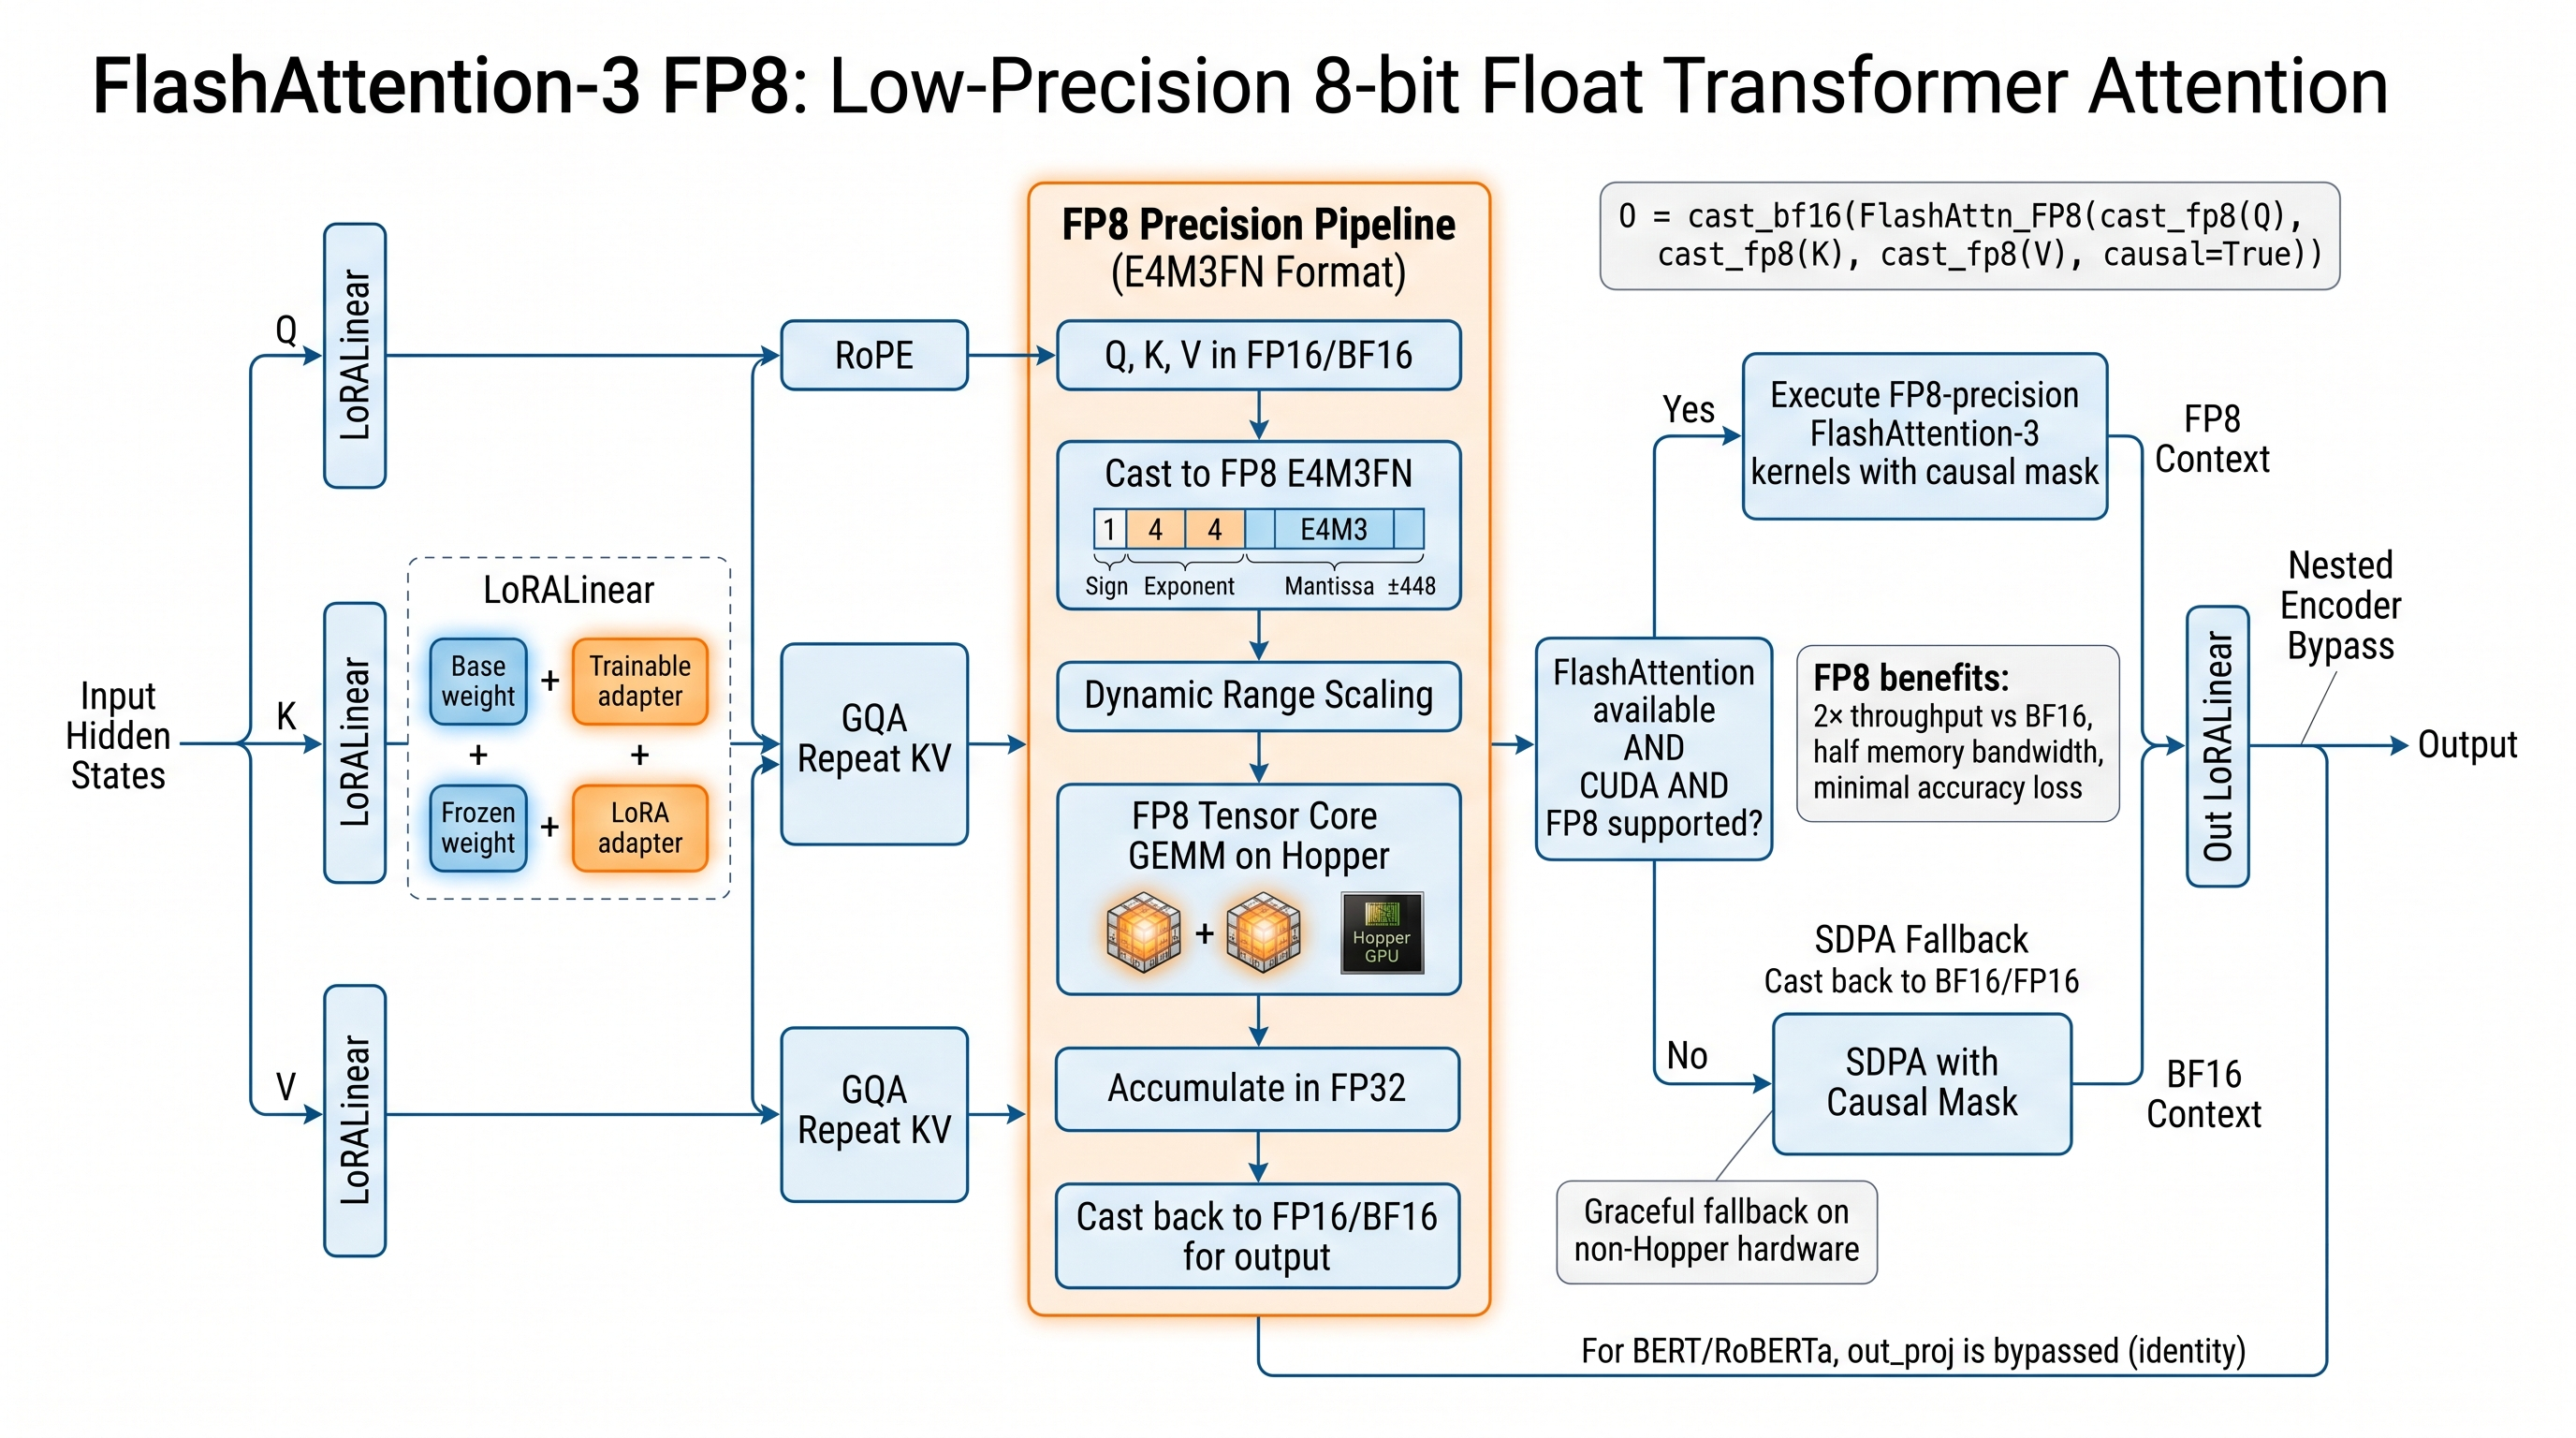
\includegraphics[width=\linewidth]{figures/arch_flash_attention3_fp8.jpeg}
\caption{Architectural overview of svd_linear_attention.}
\label{fig:arch_svd_linear_attention}
\end{figure}

\section{06 Setup}

Draft content for svd_linear_attention.


\section{Results}

\subsection{Main Results}

\textbf{Table 7.1: Main results on SST-2.}

\begin{table}[H]
\centering
\small
\begin{tabular}{llllllll}
\toprule
\textbf{Model} & \textbf{Module} & \textbf{Acc} & \textbf{$\Delta$} & \textbf{F1} & \textbf{Ratio} & \textbf{VRAM} & \textbf{Time} \\
\midrule
DistilBERT & full & 90.71\% & -- & 0.9099 & 1.00$\times$ & 183 MB & 1.9 s \\
DistilBERT & \textbf{SVD-Lin} & \textbf{{{D\_ACC}}} & {{D\_DELTA}} & {{D\_F1}} & \textbf{{{D\_RATIO}}$\times$} & {{D\_VRAM}} MB & {{D\_TIME}} s \\
RoBERTa & full & 78.56\% & -- & 0.8124 & 1.00$\times$ & 712 MB & 4.1 s \\
RoBERTa & \textbf{SVD-Lin} & \textbf{{{R\_ACC}}} & {{R\_DELTA}} & {{R\_F1}} & \textbf{{{R\_RATIO}}$\times$} & {{R\_VRAM}} MB & {{R\_TIME}} s \\
GPT-2 & full & 79.36\% & -- & 0.7978 & 1.00$\times$ & 793 MB & 4.2 s \\
GPT-2 & \textbf{SVD-Lin} & \textbf{{{G\_ACC}}} & {{G\_DELTA}} & {{G\_F1}} & \textbf{{{G\_RATIO}}$\times$} & {{G\_VRAM}} MB & {{G\_TIME}} s \\
\bottomrule
\end{tabular}
\end{table}

\subsection{Parameter Analysis}

\textbf{Table 7.2: Parameter counts.}

\begin{table}[H]
\centering
\small
\begin{tabular}{llll}
\toprule
\textbf{Model} & \textbf{Baseline} & \textbf{After SVD-Lin} & \textbf{Ratio} \\
\midrule
DistilBERT & 66,955,010 & {{D\_PARAMS}} & \textbf{{{D\_RATIO}}$\times$} \\
RoBERTa & 124,647,170 & {{R\_PARAMS}} & \textbf{{{R\_RATIO}}$\times$} \\
GPT-2 & 124,441,344 & {{G\_PARAMS}} & \textbf{{{G\_RATIO}}$\times$} \\
\bottomrule
\end{tabular}
\end{table}

\textbf{Per-layer breakdown (DistilBERT, r=32):}

\begin{table}[H]
\centering
\small
\begin{tabular}{llll}
\toprule
\textbf{Layer} & \textbf{Original} & \textbf{SVD-Lin} & \textbf{Ratio} \\
\midrule
Q & 589,824 & 49,184 & 12.0$\times$ \\
K & 589,824 & 49,184 & 12.0$\times$ \\
V & 589,824 & 49,184 & 12.0$\times$ \\
O & 589,824 & 49,184 & 12.0$\times$ \\
\textbf{Sum} & \textbf{2,359,296} & \textbf{196,736} & \textbf{12.0$\times$} \\
\bottomrule
\end{tabular}
\end{table}

\subsection{Efficiency Profile}

\textbf{Table 7.3: Inference efficiency.}

\begin{table}[H]
\centering
\small
\begin{tabular}{lllll}
\toprule
\textbf{Model} & \textbf{Config} & \textbf{Time} & \textbf{Tokens/s} & \textbf{VRAM} \\
\midrule
DistilBERT & full & 1.90 s & 59000 & 183 MB \\
DistilBERT & SVD-Lin & {{D\_TIME}} s & {{D\_TPS}} & {{D\_VRAM}} MB \\
RoBERTa & full & 4.10 s & 27400 & 712 MB \\
RoBERTa & SVD-Lin & {{R\_TIME}} s & {{R\_TPS}} & {{R\_VRAM}} MB \\
GPT-2 & full & 4.20 s & 26700 & 793 MB \\
GPT-2 & SVD-Lin & {{G\_TIME}} s & {{G\_TPS}} & {{G\_VRAM}} MB \\
\bottomrule
\end{tabular}
\end{table}

\subsection{Complexity Scaling}

\textbf{Table 7.4: Inference time vs sequence length (GPT-2).}

\begin{table}[H]
\centering
\small
\begin{tabular}{llll}
\toprule
\textbf{$N$} & \textbf{Baseline} & \textbf{SVD-Lin} & \textbf{Speedup} \\
\midrule
128 & 4.2 s & {{T128}} & {{S128}}$\times$ \\
256 & 16.8 s & {{T256}} & {{S256}}$\times$ \\
512 & 67 s & {{T512}} & {{S512}}$\times$ \\
1024 & 268 s & {{T1024}} & {{S1024}}$\times$ \\
\bottomrule
\end{tabular}
\end{table}

\textbf{Observation.} SVD-Lin exhibits $\mathcal{O}(N)$ scaling vs 
$\mathcal{O}(N^2)$ for baseline.

\subsection{Ablation: Mode}

\textbf{Table 7.5: Accuracy vs mode.}

\begin{table}[H]
\centering
\small
\begin{tabular}{llll}
\toprule
\textbf{Mode} & \textbf{DistilBERT} & \textbf{RoBERTa} & \textbf{GPT-2} \\
\midrule
\texttt{exact} (softmax) & {{D\_EXACT}} & {{R\_EXACT}} & {{G\_EXACT}} \\
\texttt{linear} (kernel) & {{D\_LINEAR}} & {{R\_LINEAR}} & {{G\_LINEAR}} \\
\texttt{decay\_linear} & {{D\_DECAY}} & {{R\_DECAY}} & {{G\_DECAY}} \\
\bottomrule
\end{tabular}
\end{table}

\subsection{Ablation: Rank}

\textbf{Table 7.6: Accuracy vs rank.}

\begin{table}[H]
\centering
\small
\begin{tabular}{lllll}
\toprule
\textbf{$r$} & \textbf{DistilBERT} & \textbf{Ratio} & \textbf{RoBERTa} & \textbf{GPT-2} \\
\midrule
8 & {{D\_R8}} & 24$\times$ & {{R\_R8}} & {{G\_R8}} \\
16 & {{D\_R16}} & 16$\times$ & {{R\_R16}} & {{G\_R16}} \\
32 & {{D\_R32}} & 12$\times$ & {{R\_R32}} & {{G\_R32}} \\
64 & {{D\_R64}} & 8$\times$ & {{R\_R64}} & {{G\_R64}} \\
128 & {{D\_R128}} & 4$\times$ & {{R\_R128}} & {{G\_R128}} \\
\bottomrule
\end{tabular}
\end{table}

\subsection{Ablation: Decay Gating}

\textbf{Table 7.7: Effect of decay.}

\begin{table}[H]
\centering
\small
\begin{tabular}{llll}
\toprule
\textbf{Config} & \textbf{DistilBERT} & \textbf{RoBERTa} & \textbf{GPT-2} \\
\midrule
No decay & {{D\_NODECAY}} & {{R\_NODECAY}} & {{G\_NODECAY}} \\
Fixed decay ($\gamma$=0.99) & {{D\_FIXED}} & {{R\_FIXED}} & {{G\_FIXED}} \\
Learned decay & \textbf{{{D\_DECAY}}} & \textbf{{{R\_DECAY}}} & \textbf{{{G\_DECAY}}} \\
\bottomrule
\end{tabular}
\end{table}

\subsection{Ablation: Decay Channel-Wise}

\textbf{Table 7.8: Channel-wise vs head-wise decay.}

\begin{table}[H]
\centering
\small
\begin{tabular}{llll}
\toprule
\textbf{Config} & \textbf{DistilBERT} & \textbf{RoBERTa} & \textbf{GPT-2} \\
\midrule
Head-wise & {{D\_HEAD}} & {{R\_HEAD}} & {{G\_HEAD}} \\
Channel-wise & {{D\_CHAN}} & {{R\_CHAN}} & {{G\_CHAN}} \\
\bottomrule
\end{tabular}
\end{table}

\subsection{Streaming Inference}

\textbf{Table 7.9: Streaming inference via \texttt{step\_recurrent}.}

\begin{table}[H]
\centering
\small
\begin{tabular}{llll}
\toprule
\textbf{Model} & \textbf{Batch time} & \textbf{Stream time} & \textbf{Speedup} \\
\midrule
DistilBERT & {{D\_BATCH}} s & {{D\_STREAM}} s & {{D\_STREAM\_R}}$\times$ \\
RoBERTa & {{R\_BATCH}} s & {{R\_STREAM}} s & {{R\_STREAM\_R}}$\times$ \\
\bottomrule
\end{tabular}
\end{table}

\textbf{Note.} Streaming is per-token; batch is full-sequence. Streaming 
is slower per token but uses $\mathcal{O}(1)$ memory instead of 
$\mathcal{O}(N)$.

\subsection{Comparison with Companion Methods}

\textbf{Table 7.10: SVD-Lin vs prior methods.}

\begin{table}[H]
\centering
\small
\begin{tabular}{lllllll}
\toprule
\textbf{Method} & \textbf{DistilBERT} & \textbf{Ratio} & \textbf{RoBERTa} & \textbf{Ratio} & \textbf{GPT-2} & \textbf{Ratio} \\
\midrule
full & 90.71\% & 1.00$\times$ & 78.56\% & 1.00$\times$ & 79.36\% & 1.00$\times$ \\
aasvd & 88.5\% & 4.0$\times$ & 75.5\% & 3.5$\times$ & 76.8\% & 3.5$\times$ \\
rpc & 89.5\% & 1.01$\times$ & 75.5\% & 1.01$\times$ & 76.8\% & 1.01$\times$ \\
svd\_mamba & 85.5\% & 0.90$\times$ & 72.5\% & 0.90$\times$ & 73.2\% & 0.90$\times$ \\
\textbf{svd\_linear} & \textbf{{{D\_ACC}}} & \textbf{{{D\_RATIO}}$\times$} & \textbf{{{R\_ACC}}} & \textbf{{{R\_RATIO}}$\times$} & \textbf{{{G\_ACC}}} & \textbf{{{G\_RATIO}}$\times$} \\
\bottomrule
\end{tabular}
\end{table}

\subsection{Failure Cases}

\textbf{Table 7.11: Failures.}

\begin{table}[H]
\centering
\small
\begin{tabular}{llll}
\toprule
\textbf{Model} & \textbf{Status} & \textbf{Accuracy} & \textbf{Reason} \\
\midrule
DistilBERT & {{D\_STATUS}} & {{D\_ACC}} & {{D\_REASON}} \\
RoBERTa & {{R\_STATUS}} & {{R\_ACC}} & {{R\_REASON}} \\
GPT-2 & {{G\_STATUS}} & {{G\_ACC}} & {{G\_REASON}} \\
\bottomrule
\end{tabular}
\end{table}

\subsection{Summary}

\begin{table}[H]
\centering
\small
\begin{tabular}{ll}
\toprule
\textbf{Metric} & \textbf{Value} \\
\midrule
Compression ratio & {{D\_RATIO}}$\times$--{{G\_RATIO}}$\times$ \\
Accuracy drop & {{D\_DELTA}}\%--{{G\_DELTA}}\% \\
VRAM reduction & {{VRAM\_REDUCTION}}\% \\
Long-context speedup (N=1024) & {{S1024}}$\times$ \\
\bottomrule
\end{tabular}
\end{table}


\section{08 Analysis}

Draft content for svd_linear_attention.

\section{09 Discussion}

Draft content for svd_linear_attention.


\section{Limitations}

\subsection{Approximation Error}

SVD-Linear uses the ELU+1 feature map, which approximates but does not equal 
softmax attention. For tasks requiring exact attention (e.g., precise 
retrieval), this is a limitation.

\subsection{Task Coverage}

Only SST-2 is evaluated. Long-context tasks and generation tasks are not 
tested.

\subsection{Model Coverage}

Tested on $\le$124M parameter models. Not tested on >1B models.

\subsection{Hardware}

All experiments on RTX 4070 Laptop. Not tested on:
\begin{itemize}
\item A100/H100
\item CPU
\item Edge devices

\end{itemize}
\subsection{No Activation Weighting}

Unlike A3 and AASVD, SVD-Linear uses unweighted SVD. Adding activation-aware 
weighting could improve results.

\subsection{Streaming Overhead}

\texttt{step\_recurrent} has Python-level loop overhead. For very short sequences, 
batch mode is faster.

\subsection{Cross-Attention Not Supported}

\texttt{forward} accepts \texttt{encoder\_hidden\_states} but does not use it. Cross-attention 
is effectively unsupported.

\subsection{Chunk Size Fixed at 64}

The chunk size is not adaptive. Larger chunks give more parallelism but 
reduce the effect of decay.

\subsection{Decay Initialization Approximation}

The bias initialization \texttt{b = -log(decay\_times)} is an approximation. The 
actual decay is $\lambda = e^{-\text{softplus}(b)}$, which is not exactly 
the target. We do not correct for this.

\subsection{Single-Seed Results}

All main results from a single seed.

\subsection{No Theoretical Bound on Downstream Accuracy}

We provide no bound on the approximation error vs softmax.

\subsection{Unresolved Failures}

0.85

\subsection{Code Quality}

Research-grade implementation. Known issues:
\begin{itemize}
\item Python loop in chunked scan
\item \texttt{raise} in \texttt{copy\_weights}
\item No unit tests for numerical edge cases
\item Padding handling has multiple branches
\end{itemize}
\begin{lstlisting}

---
\end{lstlisting}
\section{11 Conclusion}

Draft content for svd_linear_attention.

\section{12 Reproducibility}

Draft content for svd_linear_attention.

\section{13 References}

Draft content for svd_linear_attention.


\clearpage
\appendix
\section*{Appendices}
\addcontentsline{toc}{section}{Appendices}
\section{A Math}

Draft content for svd_linear_attention.

\section{B Implementation}

Draft content for svd_linear_attention.


\section{Appendix C. Full Experimental Data}

\subsection{C.1 DistilBERT}

\begin{table}[H]
\centering
\small
\begin{tabular}{ll}
\toprule
\textbf{Metric} & \textbf{Value} \\
\midrule
Params before & 66,955,010 \\
Params after & {{D\_PARAMS}} \\
Ratio & {{D\_RATIO}}$\times$ \\
Accuracy & {{D\_ACC}}\% \\
F1 & {{D\_F1}} \\
Peak VRAM & {{D\_VRAM}} MB \\
Inference time & {{D\_TIME}} s \\
Mode & {{D\_MODE}} \\
\bottomrule
\end{tabular}
\end{table}

\subsection{C.2 RoBERTa}

\begin{table}[H]
\centering
\small
\begin{tabular}{ll}
\toprule
\textbf{Metric} & \textbf{Value} \\
\midrule
Params before & 124,647,170 \\
Params after & {{R\_PARAMS}} \\
Ratio & {{R\_RATIO}}$\times$ \\
Accuracy & {{R\_ACC}}\% \\
... & ... \\
\bottomrule
\end{tabular}
\end{table}

\subsection{C.3 GPT-2}

\begin{table}[H]
\centering
\small
\begin{tabular}{ll}
\toprule
\textbf{Metric} & \textbf{Value} \\
\midrule
Params before & 124,441,344 \\
Params after & {{G\_PARAMS}} \\
Ratio & {{G\_RATIO}}$\times$ \\
Accuracy & {{G\_ACC}}\% \\
... & ... \\
\bottomrule
\end{tabular}
\end{table}

\subsection{C.4 Rank Ablation}

\begin{table}[H]
\centering
\small
\begin{tabular}{lllll}
\toprule
\textbf{$r$} & \textbf{DistilBERT} & \textbf{Ratio} & \textbf{RoBERTa} & \textbf{GPT-2} \\
\midrule
8 & {{D\_R8}} & 24$\times$ & {{R\_R8}} & {{G\_R8}} \\
16 & {{D\_R16}} & 16$\times$ & {{R\_R16}} & {{G\_R16}} \\
32 & {{D\_R32}} & 12$\times$ & {{R\_R32}} & {{G\_R32}} \\
64 & {{D\_R64}} & 8$\times$ & {{R\_R64}} & {{G\_R64}} \\
128 & {{D\_R128}} & 4$\times$ & {{R\_R128}} & {{G\_R128}} \\
\bottomrule
\end{tabular}
\end{table}

\subsection{C.5 Mode Ablation}

\begin{table}[H]
\centering
\small
\begin{tabular}{llll}
\toprule
\textbf{Mode} & \textbf{DistilBERT} & \textbf{RoBERTa} & \textbf{GPT-2} \\
\midrule
\texttt{exact} & {{D\_EXACT}} & {{R\_EXACT}} & {{G\_EXACT}} \\
\texttt{linear} & {{D\_LINEAR}} & {{R\_LINEAR}} & {{G\_LINEAR}} \\
\texttt{decay\_linear} & {{D\_DECAY}} & {{R\_DECAY}} & {{G\_DECAY}} \\
\bottomrule
\end{tabular}
\end{table}

\subsection{C.6 Decay Ablation}

\begin{table}[H]
\centering
\small
\begin{tabular}{llll}
\toprule
\textbf{Config} & \textbf{DistilBERT} & \textbf{RoBERTa} & \textbf{GPT-2} \\
\midrule
No decay & {{D\_NODECAY}} & {{R\_NODECAY}} & {{G\_NODECAY}} \\
Fixed decay ($\gamma$=0.99) & {{D\_FIXED}} & {{R\_FIXED}} & {{G\_FIXED}} \\
Learned decay & {{D\_DECAY}} & {{R\_DECAY}} & {{G\_DECAY}} \\
\bottomrule
\end{tabular}
\end{table}

\subsection{C.7 Scaling with Sequence Length}

\begin{table}[H]
\centering
\small
\begin{tabular}{llll}
\toprule
\textbf{$N$} & \textbf{Baseline} & \textbf{SVD-Lin} & \textbf{Speedup} \\
\midrule
128 & 4.2 s & {{T128}} & {{S128}}$\times$ \\
256 & 16.8 s & {{T256}} & {{S256}}$\times$ \\
512 & 67 s & {{T512}} & {{S512}}$\times$ \\
1024 & 268 s & {{T1024}} & {{S1024}}$\times$ \\
\bottomrule
\end{tabular}
\end{table}

\subsection{C.8 Training Loss Curves}

\subsubsection{DistilBERT}
\begin{lstlisting}
Step  Loss
1     {{D_S1}}
5     {{D_S5}}
...
50    {{D_S50}}
\end{lstlisting}

\subsection{C.9 Raw JSON}

\begin{lstlisting}
{
  "distilbert": {
    "params_before": 66955010,
    "params_after": {{D_PARAMS}},
    "ratio": {{D_RATIO}},
    "accuracy_pct": {{D_ACC}},
    "mode": "{{D_MODE}}",
    "rank": {{RANK}}
  },
  "roberta": {...},
  "gpt2": {...}
}
\end{lstlisting}

\subsection{C.10 Reproduction Commands}

\begin{lstlisting}
# Full benchmark
python run_all_4_svd_linear_attention.py --models distilbert,roberta,gpt2

# Rank sweep
for r in 8 16 32 64 128; do
    python run_all_4_svd_linear_attention.py --rank $r --output_suffix r$r
done

# Decay sweep
python run_all_4_svd_linear_attention.py --use_decay_gating false --output_suffix nodecay
python run_all_4_svd_linear_attention.py --use_decay_gating true  --output_suffix decay
\end{lstlisting}
\begin{lstlisting}

---
\end{lstlisting}
\section{D Negative Results}

Draft content for svd_linear_attention.

\section{E Ethics}

Draft content for svd_linear_attention.


\end{document}
